\documentclass[11pt]{article}
\linespread{1.25}

\usepackage[top = 2cm, right=2cm, left=2cm]{geometry}
\usepackage{graphicx}

\usepackage[section]{placeins}
\usepackage[hidelinks, urlcolor=blue]{hyperref}
\usepackage{float} % for image position in exatly where you want
\usepackage[perpage, stable]{footmisc}
\usepackage{amsmath}
\usepackage{titling}


\usepackage{xepersian}
\settextfont{B Nazanin}
\setlatinmonofont{CMU Serif}
%\setlatinmonofont{Times New Roman}
\setlatintextfont{Times New Roman}


% Set Latin Modern font for the bullets in itemizea
\newfontfamily\latinbullet{Latin Modern Roman}





% Commands
\newcommand{\column}[1]{\lr{\textit{#1}}}
\renewcommand{\labelitemi}{{\latinbullet\textbullet}} % Use the bullet from Latin Modern font

% Custom title page setup
\makeatletter
\def\maketitle{
	\begin{titlepage}
		\begin{center}
			\vspace*{2cm}
			
			{\Large\bfseries درس یادگیری ماشین\par}
			\vspace{2cm}
			
			{\Huge\bfseries گزارش تکلیف
				\lr{Neural Networks}\par}
			\vspace{3cm}
			
			{\large\bfseries استاد درس:\par}
			{\large دکتر افتخاری\par}
			\vspace{1.5cm}
			
			{\large\bfseries نگارش:\par}
			{\large امیرحسین ابوالحسنی\par}
			{\large شماره دانشجویی: 400405003\par}
			\vspace{2cm}
			
			\vfill  % pushes the date to bottom
			
			{\large\bfseries پاییز \lr{1403}}
		
		\end{center}
	\end{titlepage}
	\setcounter{page}{1}
}
\makeatother


\begin{document}
	\maketitle	
	\tableofcontents
	\newpage
	\section{مقدمه}
	یکی از بهترین کتابخانه‌ها برای پیاده‌سازی شبکه‌های عصبی، کتابخانه
	\lr{Pytorch}	
	می‌باشد. در این تکلیف به پیاده‌سازی شبکه عصبی ساده برای تسک طبقه بندی روی دیتاست 
	\lr{MNIST}
	 پرداخته می‌شود.
	 \section{معماری شبکه}
	 برای معماری شبکه عصبی استفاده شده، از دو لایه 
	 \lr{Perceptron}
	 به همراه تابع فعال ساز 
	 \lr{ReLU}
	 استفاده شده است.
	 \begin{figure}[H]
	 	\centering
	 	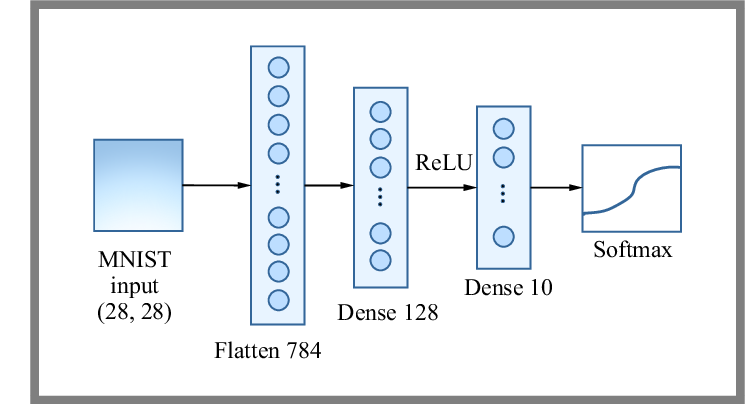
\includegraphics{figs/arch}
	 	\caption{معماری شبکه عصبی}
	 	\label{fig: arch}
	 \end{figure}
	 \section{بهینه‌ساز و تابع هزینه}
	 برای آموزش مدل از بهینه‌ساز 
	 \lr{Adam}
	 استفاده شده است.
	 \begin{latin}
	 \begin{align*}
	 	m_t &= \beta_1 \cdot m_{t-1} + (1 - \beta_1) \cdot g_t \\
	 	v_t &= \beta_2 \cdot v_{t-1} + (1 - \beta_2) \cdot g_t^2 \\
	 	\hat{m}_t &= \frac{m_t}{1 - \beta_1^t} \\
	 	\hat{v}_t &= \frac{v_t}{1 - \beta_2^t} \\
	 	\theta_t &= \theta_{t-1} - \frac{\alpha \cdot \hat{m}_t}{\sqrt{\hat{v}_t} + \epsilon}
	 \end{align*}
	 
	 Where:
	 \begin{itemize}
	 	\item $m_t$: First moment estimate (mean of gradients)
	 	\item $v_t$: Second moment estimate (uncentered variance of gradients)
	 	\item $g_t$: Gradient at time step $t$
	 	\item $\beta_1, \beta_2$: Exponential decay rates
	 	\item $\alpha$: Learning rate
	 	\item $\epsilon$: Small constant to prevent division by zero
	 	\item $\theta_t$: Updated parameter
	 \end{itemize}
	\end{latin}
	تابع هزینه‌ای که برای این مدل در نظر گرفته شده، به علت نوع تسک که طبقه بندی است، 
	\lr{Cross Entropy}
	می‌باشد.
	 \section{آموزش مدل}
	 مدل با پارامترهای جدول
	 \ref{tbl: hyper params}
	 آموزش دیده است. 
	 \begin{table}[H]
	 	\centering
	 	\begin{tabular}{|c|c|}
	 		\hline
	 		نام هایپر پارامتر & مقدار\\
	 		\hline
	 		\lr{Epochs} & 5\\
	 		\hline
	 		\lr{Learning Rate} & 001.0\\
	 		\hline
	 		\lr{Batch Size} & 128\\
	 		\hline
	 	\end{tabular}
	 \caption{مقادیر هایپر پارامترهای مدل}	 	
	 \label{tbl: hyper params}	 
	 \end{table}
	 \section{ارزیابی مدل}
	 پس از آموزش مدل نوبت به ارزیابی آن می رسد. دو متریک دقت و 
	 \lr{F1 Score}
	 برای ارزیابی عملکرد مدل استفاده شده است.
	 \begin{table}[H]
	 	\centering
	 	\begin{tabular}{|c|c|}
	 		\hline
	 		معیار & مقدار\\
	 		\hline
	 		دقت & 69.0\\
	 		\hline
	 		\lr{F1 Score} & 698.0\\
	 		\hline
	 	\end{tabular}
	 	\caption{نمرات ارزیابی مدل ارائه شده}	 	
	 	\label{tbl: model res}	 
	 \end{table}
	 همچنین در شکل
	 \ref{fig: confmat}
	 ، ماتریس سردرگمی نشان داده شده است.
	 \begin{figure}[H]
	 	\centering
	 	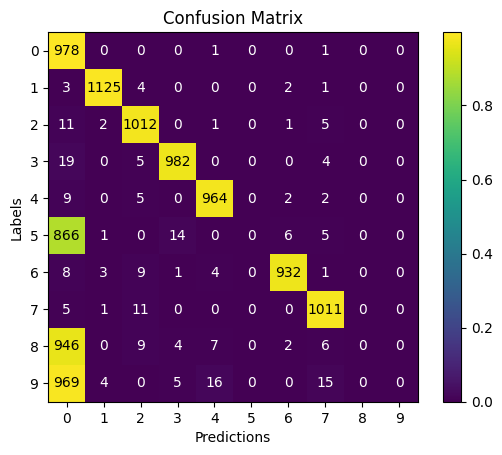
\includegraphics[scale=0.5]{figs/confmat}
	 	\caption{ماتریس سردرگمی}
	 	\label{fig: confmat}
	 \end{figure}
	 \newpage
	 \section{خروجی مدل}
	 نمونه ای از خروجی مدل در شکل
	 \ref{fig: preds}
	  قابل مشاهده است.
	 \begin{figure}[H]
	 	\centering
	 	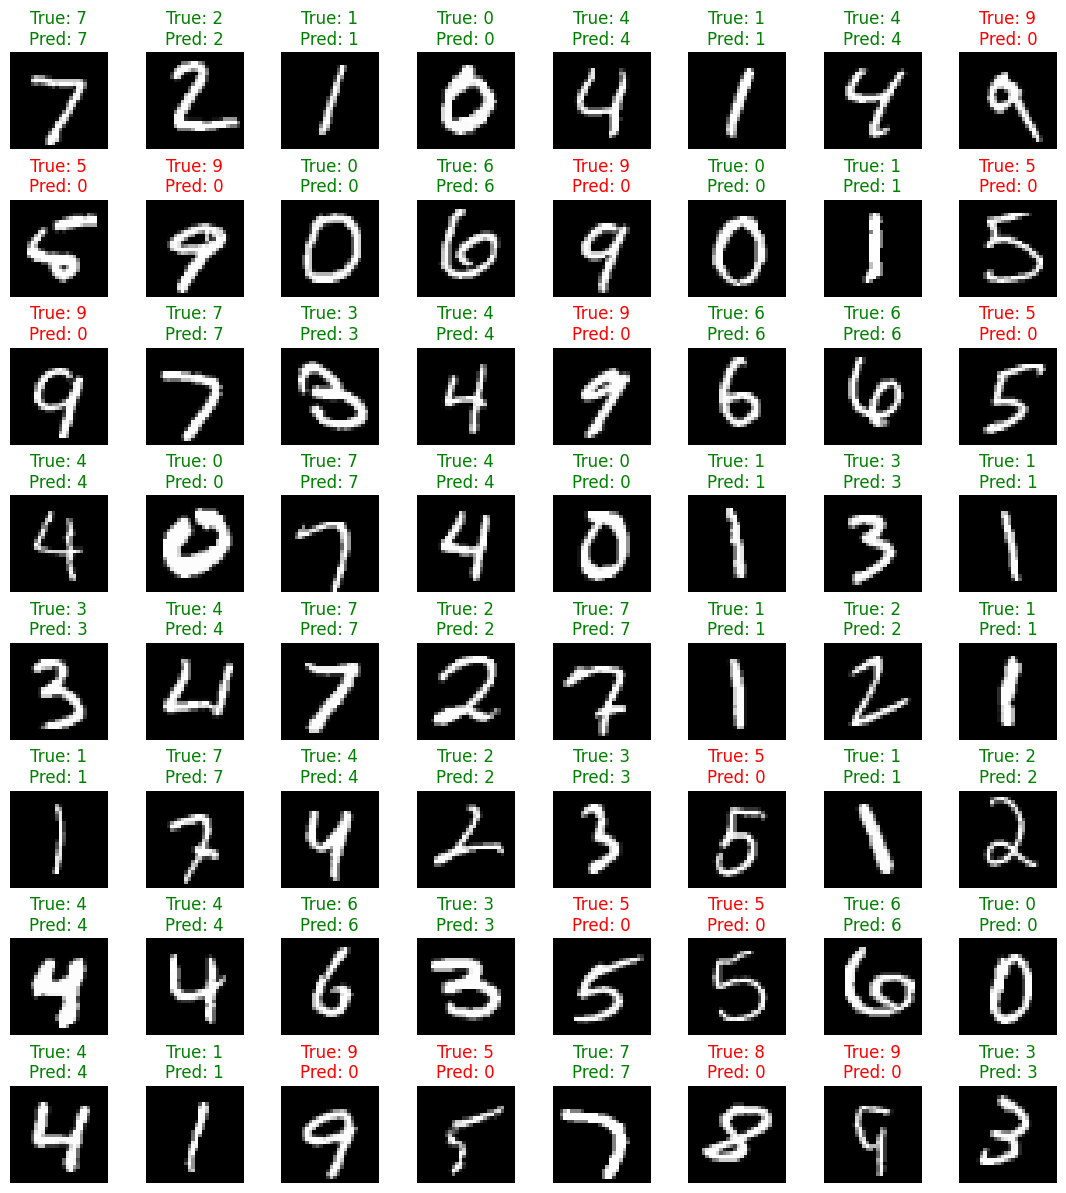
\includegraphics[scale=0.4]{figs/pred}
	 	\caption{خروجی مدل برای یک دسته از داده تست}
	 	\label{fig: preds}
	 \end{figure}
\end{document}